\RequirePackage[T1]{fontenc}
\documentclass[conference,letterpaper]{IEEEtran}
\usepackage{cite}
\usepackage{float,stfloats}
\setcounter{dblbotnumber}{2}

\usepackage{amsmath,amssymb,dsfont,graphicx,array,booktabs}
\usepackage{mathptmx}
\usepackage[hidelinks]{hyperref}
\title{Do Frozen Hand-Pose Classifiers Preserve Their Decisions Under EMG-Predicted Inputs?}
\author{\IEEEauthorblockN{Boyan Dong}\IEEEauthorblockA{School of Biological Science and Medical Engineering, Southeast University, Nanjing, China\\yan494815@gmail.com}}

\begin{document}
\flushbottom
\maketitle
\typeout{STANDARD-METRICS: BASELINE=\the\baselineskip; WIDTH=\the\textwidth; HEIGHT=\the\textheight; COLUMN=\the\columnwidth}
\begin{abstract}

Estimating hand joint angles from electromyography (EMG) allows existing pose-based gesture classifiers to be reused without retraining on EMG data. However, replacing directly measured poses with EMG-predicted poses can still alter a fixed classifier's output---an event we term a \textit{decision flip}. We evaluate this risk using one frozen EMG-to-pose estimator and six frozen pose classifiers across four public datasets ($N = 80$ participants). Without filtering, input substitution flipped 16.43\% to 43.05\% of baseline classifier decisions. Applying a learned selective gating model (\textit{full-feature ranking}) to retain the top 30\% most reliable predictions reduced median overall decision disagreement by 1.87--4.65 percentage points compared to a baseline boundary-distance filter. Crucially, however, improving overall agreement did not guarantee consistent decisions across individual gesture classes, because filtering can retain easy-to-predict classes while discarding harder ones. For instance, in one task (\textit{SHOW instruction}), overall disagreement improved by 2.61 percentage points, whereas class-balanced disagreement (weighting all classes equally) worsened by 20.88 percentage points across the same 79 evaluable participants. In another task (\textit{DB9 posture}), retaining 30\% of predictions depleted per-class sample counts, reducing the number of participants with complete class support from 22/80 to just 3/80. These results reveal a critical evaluation blind spot: lowering aggregate disagreement can mask severe class-balanced degradation and sample depletion. Jointly reporting overall disagreement, class-balanced disagreement, and evaluable class support is therefore essential when reusing pose classifiers with EMG inputs.

\end{abstract}

\section{INTRODUCTION}

Surface electromyography (EMG) is widely used to decode hand movements and gestures directly from muscle activity. Typically, adapting a direct EMG classifier to a new gesture set requires collecting new labeled EMG data and retraining the model. A modular alternative is to first estimate hand pose---represented by finger-joint angles---from EMG, and then pass those predicted angles to downstream classifiers already trained on directly measured pose data (e.g., from sensor gloves or motion-capture cameras) \cite{ref1}. In principle, a single shared EMG-to-pose model could support multiple downstream classification tasks without task-specific EMG retraining.

Yet matching a classifier's input format does not guarantee preserving its decisions. Even when pose estimation error is small on average, angle deviations can push an input across a classifier's decision boundary. For example, as illustrated in Fig. 1, a frozen gesture classifier might recognize a measured hand pose as an "open hand" (class A), but misclassify the corresponding EMG-predicted pose as a "fist" (class B). We call this change a \textit{decision flip}: input substitution alters the downstream classifier's output, regardless of whether either prediction matches an independently verified action label. Evaluating whether EMG-predicted poses can safely replace measured poses therefore requires examining downstream decision flips directly, rather than relying solely on pose reconstruction error.

Previous work has investigated EMG-based hand pose estimation \cite{ref1}, pose-guided EMG representation learning \cite{ref2, ref3}, and confidence-based rejection in myoelectric control or selective prediction \cite{ref4, ref5, ref6}. While selective gating---rejecting uncertain predictions to retain only reliable ones---can reduce decision flips overall, it introduces a subtle risk across individual gesture classes. If a gate preferentially retains easy-to-agree gestures (e.g., open hands) while rejecting harder ones (e.g., fists), \textit{overall} agreement across all retained samples will appear to improve, even as agreement worsens when classes are weighted equally or as certain classes lose too many samples to be evaluated reliably.

To investigate this issue directly, we hold one upstream EMG-to-pose estimator \cite{ref1} and six downstream pose classifiers \cite{ref7,ref8,ref9,ref10} frozen to examine three connected questions: (1) how often substituting EMG-predicted poses for measured poses flips frozen downstream decisions; (2) whether learned offline gating reduces these flips over boundary-distance filtering at matched retention rates; and (3) whether improvements in overall agreement extend across individual reference classes without depleting per-class sample support. Together, these questions establish a rigorous retrospective evaluation of decision preservation across modular EMG-to-pose pipelines.

\section{METHODS}

\subsection{Frozen Pose Classifiers and Input Substitution}

A \textit{frozen pose classifier} is a pretrained gesture classifier whose parameters and source standardization remain fixed. As shown in Fig. 1, we pass paired measured poses and EMG-predicted poses (from the frozen \textrm{VEMG2Pose} estimator \cite{ref1}) through six frozen LDA classifiers across four public datasets: posture and grasp classification from DB9 \cite{ref7} and CeTI-Age \cite{ref8}, instruction classification from SHOW3D \cite{ref9}, and movement-phase classification from KIN-MUS UJI \cite{ref10}. The estimator and each classifier connect via a fixed eight-joint adapter in radians: thumb MCP/IP, index MCP/PIP, middle/ring MCP, and little-finger MCP/PIP (native indices 2, 3, 5, 6, 9, 13, 17, 18) \cite{ref1}. Target pose and reference streams share a 1790-sample crop aggregated into non-overlapping 40-sample means, yielding aligned $\approx$20-ms eight-dimensional pose vectors (time-stamped at the block end) that are standardized using fixed source statistics and fed directly into each static LDA classifier (native source training windows: 32 frames or 0.808 s for CeTI; $\approx$0.8-s windows for SHOW and KIN).

\begin{figure}[!t]
\centering
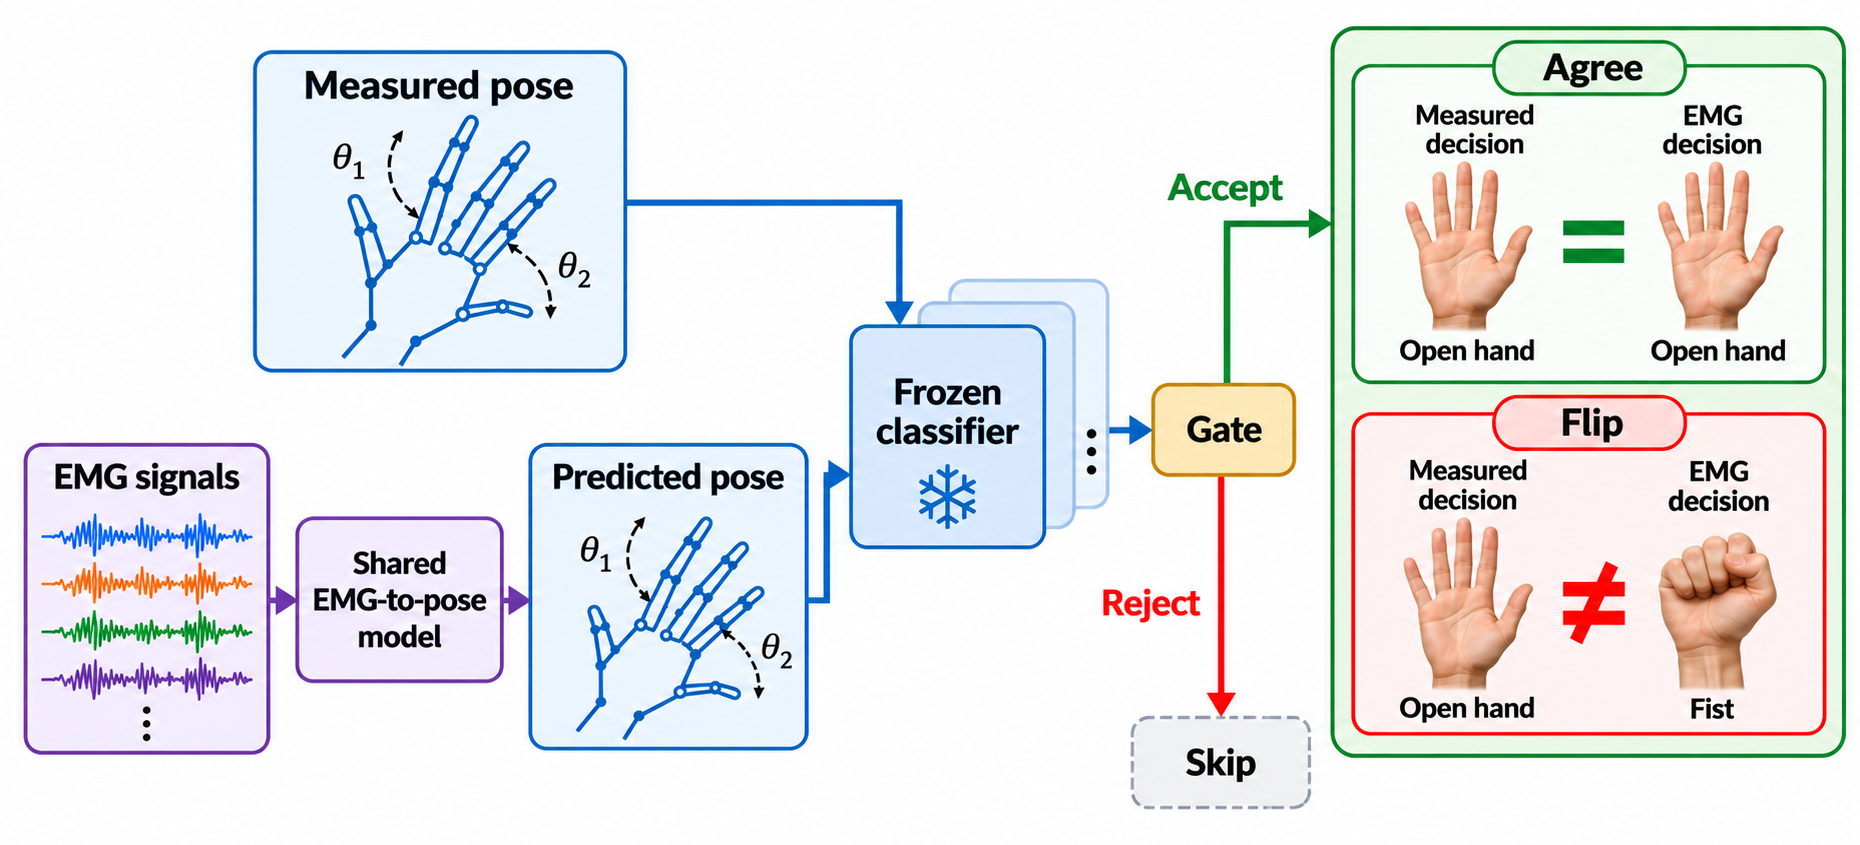
\includegraphics[width=\linewidth]{figures/fig1_frozen_classifier_gate.png}
\caption{Evaluating decision preservation across frozen pose classifiers under EMG input substitution. Measured and EMG-predicted poses pass through the same frozen classifier; a flip occurs when their outputs differ. An offline gate filters predictions using predicted-pathway features.}
\label{fig:substitution}
\end{figure}

To verify baseline integrity on measured poses, we reproduced source-domain leave-one-subject-out (LOSO) evaluations against archived out-of-fold predictions. Across tasks with $K_i \in \{3, 8\}$ classes (uniform guessing baselines: 12.50\% for $K_i=8$, 33.33\% for $K_i=3$), reproduced balanced accuracies were 74.79\% for DB9 posture ($K_i=8$), 85.50\% for DB9 grasp ($K_i=3$), 58.56\% for CeTI posture ($K_i=8$), 72.25\% for CeTI grasp ($K_i=3$), 100.00\% for SHOW instruction ($K_i=3$: finger-guns, thumbs-up-down, pinch-and-zoom; recording-level LOSO across 16 participants and 60 recordings by averaging within-recording window discriminant scores), and 56.17\% for KIN phase ($K_i=3$).

\subsection{Decision Flips, Coverage, and Reference-Class Support}

For classifier $i$, participant $u$, and block $t$, measured pose $q_{u,t}$ and EMG-predicted pose $\hat{q}_{u,t}$ define the binary flip indicator:

\begin{equation}
F_{u,t}^{(i)} = \mathbf{1}\left[C_i(\hat{q}_{u,t}) \neq C_i(q_{u,t})\right].
\end{equation}

Let $V_u$ be prediction-valid blocks, $P_u \subseteq V_u$ those with valid measured references, and $A_u \subseteq V_u$ blocks accepted by the gate. Overall (block-pooled) disagreement ($U$) and coverage ($Y$) are:

\begin{equation}
U_u^{(i)} = \frac{\sum_{t \in A_u \cap P_u} F_{u,t}^{(i)}}{|A_u \cap P_u|}, \quad Y_u = \frac{|A_u \cap V_u|}{|V_u|},
\end{equation}

where $U_u^{(i)}$ is undefined if $A_u \cap P_u = \emptyset$. Given the measured-pose reference-class support set

\begin{equation}
R_{u,k}^{(i)} = \{t \in P_u : C_i(q_{u,t}) = k\},
\end{equation}

class-balanced disagreement ($B$) averages within-class flip rates equally across all $K_i$ classes:

\begin{equation}
B_u^{(i)} = \frac{1}{K_i} \sum_{k=1}^{K_i} \frac{\sum_{t \in A_u \cap R_{u,k}^{(i)}} F_{u,t}^{(i)}}{|A_u \cap R_{u,k}^{(i)}|}.
\end{equation}

$B_u^{(i)}$ is reported only when all $K_i$ classes have $\vert{}R_{u,k}^{(i)}\vert{} \ge 30$ before gating and $\vert{}A_u \cap R_{u,k}^{(i)}\vert{} \ge 30$ afterward; otherwise $B_u^{(i)}$ is undefined (unsupported classes are never silently excluded).

\subsection{Selective Gating Methods}

Selective gating filters which predicted-input decisions are accepted using predicted-pathway features only. We compare three strategies: \textit{1) Boundary}, ranking inputs by distance to the nearest competing decision boundary; \textit{2) Score-only}, using predicted class, discriminant scores, score gap, entropy, and boundary distance; and \textit{3) Full}, extending \textit{Score-only} with the eight predicted joint angles, source-fitted LDA Fisher coordinates, and two variation descriptors across four fixed EMG views (original, $0.97\times$/$1.03\times$ amplitude scaling, and Gaussian noise at $0.005\times$ whole-record RMS).

Learned gates are trained on up to 5,000 deterministically sampled paired blocks per development participant to fit a weighted binary flip-risk proxy. Following development selection, our primary overall-risk configuration (\textrm{/U}, i.e., \textrm{Score-only/U} and \textrm{Full/U}) uses histogram gradient boosting (100 iterations, depth 3, learning rate 0.1, L2 penalty 1, seed 0) with participant and flip-state balancing. A class-balanced configuration (\textrm{/B}, e.g., \textrm{Full/B}) adds reference-class weighting via standardized logistic regression ($C=1$, 300 iterations, seed 0); because \textrm{/U} and \textrm{/B} vary both model family and weights, their differences reflect the combined configuration.

\begin{table*}[!t]
\centering
\caption{Overall Disagreement and Paired Gains at 30\% Offline Retention (N80)}
\label{tab:overall}
\begingroup
\small
\setlength{\tabcolsep}{3pt}
\renewcommand{\arraystretch}{1.05}
\begin{tabular}{lrrrrl}
\toprule
Classifier (Task) & No Gate $U$ & Boundary $U$ & Score-only/U $U$ & Full/U $U$ & Paired Boundary--Full/U (95\% CI)\\
\midrule
DB9 posture ($K=8$) & 38.91 & 21.95 & 17.29 & 16.00 & 4.651 [2.784, 6.505]\\
DB9 grasp ($K=3$) & 18.37 & 6.67 & 4.87 & 3.46 & 1.867 [1.431, 2.371]\\
CeTI posture ($K=8$) & 43.05 & 24.73 & 21.87 & 20.77 & 3.973 [2.918, 5.312]\\
CeTI grasp ($K=3$) & 41.10 & 31.59 & 29.60 & 25.65 & 4.261 [2.214, 6.446]\\
SHOW instruction ($K=3$) & 16.43 & 6.93 & 6.29 & 4.10 & 2.591 [1.655, 3.006]\\
KIN phase ($K=3$) & 22.32 & 5.95 & 3.81 & 3.66 & 2.107 [1.300, 3.302]\\
\bottomrule
\end{tabular}
\par\smallskip
\begin{minipage}{\linewidth}\footnotesize
No Gate retains 100\% of valid blocks; selective gates retain 30\%. Columns show participant median overall disagreement U (\%; lower is better) and within-participant Boundary-minus-Full/U reductions (pp; higher is better) with pointwise 95\% bootstrap intervals (n = 80).
\end{minipage}
\endgroup

\end{table*}

\begin{figure*}[!b]
\centering
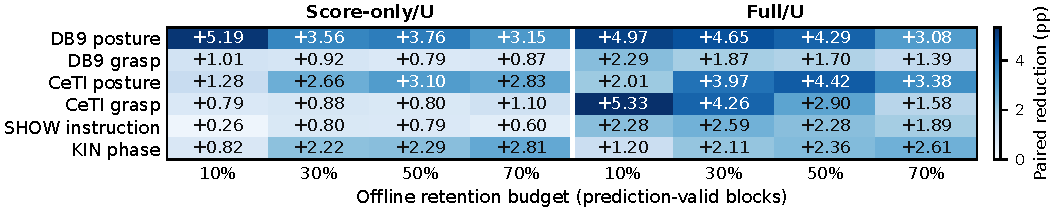
\includegraphics[width=0.85\linewidth]{figures/fig2_N80_ranking.pdf}
\caption{Median within-participant reductions in overall disagreement (pp) relative to Boundary across six frozen classifiers at four offline retention budgets in N80 (n = 80; positive values indicate improvement).}
\label{fig:ranking}
\end{figure*}

\subsection{Gating and Evaluation Protocols}

Our primary protocol compares gates at matched offline retention budgets $r \in \{10\%, 30\%, 50\%, 70\%\}$ ($\lceil r\vert{}V_u\vert{} \rceil$ blocks accepted per participant using deterministic tie handling); \textrm{No Gate} accepts 100\%. To test cross-user threshold transferability, we also partition 19 development participants into 13 for fitting, 3 for threshold selection, and 3 for diagnostic validation. A fixed threshold is feasible if it achieves $\le 10\%$ disagreement across all threshold-selection participants with $> 10\%$ median coverage (plus complete support for \textrm{/B}); infeasible settings use a 30\% fallback without being counted as feasible.

\subsection{Cohorts and Statistical Analysis}

We evaluate two cohorts disjoint from the 19 development participants: \textbf{N80} (80 participants; 7,111,408 valid pairs, primary) and \textbf{A20} (20 participants; 1,650,789 pairs, secondary). Because public upstream metadata record training files for 70/80 N80 and 16/20 A20 participants without specifying exact checkpoint membership, our results characterize the specified frozen pipelines rather than certified unseen-user generalization. Using participants as statistical units, we compute within-participant method differences first and report across-participant medians with descriptive 95\% confidence intervals (CIs) from 10,000 participant-level bootstrap resamples. Balanced comparisons ($B$) include only jointly evaluable participants.

\section{RESULTS}

\begin{figure*}[!t]
\centering
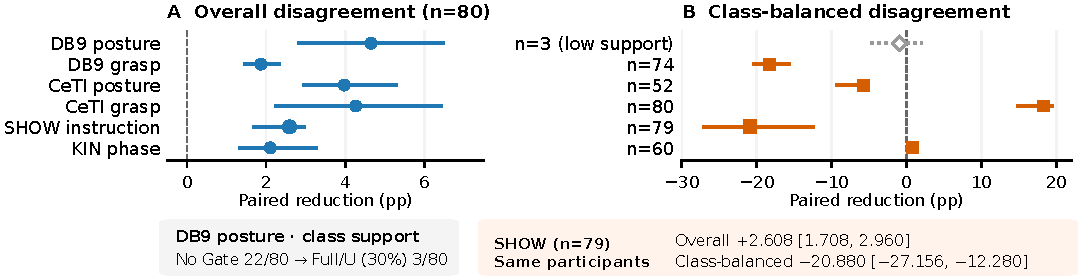
\includegraphics[width=0.85\linewidth]{figures/fig3_class_fidelity.pdf}
\caption{Paired Boundary-minus-Full/U reductions (pp) at 30\% retention for (A) overall (n = 80) and (B) class-balanced disagreement (jointly evaluable counts n shown). Positive values indicate improvement. SHOW reverses direction (n = 79), and DB9 posture support drops from 22/80 to 3/80.}
\label{fig:fidelity}
\end{figure*}

\subsection{Baseline Decision Flips Under Pose Substitution}

Without gating (\textrm{No Gate}), N80 participant-median overall disagreement ($U$) at the 20-ms scale ranged from 16.43\% for SHOW instruction to 43.05\% for CeTI posture (Table I). In a window-sensitivity test aggregating inputs into 800-ms windows, median \textrm{No Gate} disagreement decreased modestly---to 12.84\% (SHOW), 15.32\% (DB9 grasp), 21.37\% (KIN), 35.08\% (DB9 posture), 39.34\% (CeTI grasp), and 41.75\% (CeTI posture)---showing that while flip rates depend on aggregation scale, substantial flips persist at wider windows. However, 800-ms aggregation sharply reduces total blocks, shrinking 30\%-retention \textrm{Full/U} complete class support from 79 to 4 participants in SHOW and from 3 to 0 in DB9 posture. At the primary 20-ms scale, baseline support ($\ge 30$ blocks per class) was met in 22/80 participants for DB9 posture and 79/80 for KIN phase, versus 80/80 for the other four tasks; in DB9 posture, reference output label 3 had a median of only 3 blocks per participant ($\ge 30$ blocks in 22/80; zero in 34/80).

\subsection{Selective Gating Across Frozen Classifiers}

At 30\% retention, \textrm{Full/U} reduced overall disagreement across all six classifiers in N80 relative to \textrm{Boundary}, with median within-participant reductions ranging from 1.867 pp for DB9 grasp (95\% CI: [1.431, 2.371]) to 4.651 pp for DB9 posture ([2.784, 6.505]) (Table I). Across all four budgets (10\%--70\%), \textrm{Full/U} improved over \textrm{Boundary} in all 24 task--budget settings in both N80 (Fig. 2) and A20, and outperformed \textrm{Score-only/U} in 23/24 N80 and 22/24 A20 settings (e.g., by 3.790 pp, [2.774, 4.691] in N80 CeTI grasp at 30\% retention). Conditional gains from multi-view EMG perturbations alone were small (0.040--0.226 pp at 30\% retention; 4/6 CIs crossing zero). The secondary A20 cohort thus showed the same direction of \textrm{Full/U} improvement over \textrm{Boundary} as N80 at each of the four retention budgets. In the cross-user fixed-threshold audit, only 4/24 \textrm{Score-only} (0/12 \textrm{Score-only/B}) and 3/6 \textrm{Full/U} (0/6 \textrm{Full/B}) configurations met feasibility criteria.

\subsection{Class-Balanced Disagreement and Reference Support Depletion}

Lowering overall disagreement did not guarantee uniform preservation across reference classes at 30\% retention (Fig. 3). In SHOW instruction, across the 79 jointly evaluable participants, \textrm{Full/U} reduced overall disagreement by a median of 2.608 pp ([1.708, 2.960]; 2.591 pp across all $n=80$ in Table I), whereas class-balanced disagreement ($B$) worsened by 20.880 pp ([12.280, 27.156]). Applying the class-weighted \textrm{Full/B} gate at 30\% retention reversed this trade-off in SHOW---improving $B$ by 5.533 pp ($n=80$) while worsening $U$ by 6.419 pp ($n=80$)---yet did not prevent class-balanced degradation in all tasks (e.g., KIN phase $B$ still worsened by 8.677 pp, $n=52$). Conversely, under \textrm{Full/U}, CeTI grasp improved in both $U$ (+4.261 pp) and $B$ (+18.31 pp, $n=80$). Furthermore, selective filtering reduced DB9 posture complete class support from 22/80 (\textrm{No Gate}) to just 3/80 under \textrm{Full/U} at 30\% retention (Fig. 3).

\section{DISCUSSION}

Format compatibility does not guarantee decision preservation across modular pose interfaces: substituting EMG-predicted poses flipped 16.43\%--43.05\% of baseline decisions, and while selective gating consistently reduced aggregate disagreement, class-level outcomes diverged across tasks. Because overall disagreement ($U$) pools accepted blocks by frequency, a gate can lower $U$ by retaining frequent, easy-to-agree classes while rejecting harder ones. Class-balanced disagreement ($B$) exposes this bias, moving opposite to $U$ in SHOW instruction (+2.61 pp overall gain vs. $-20.88\text{ pp}$ balanced worsening under \textrm{Full/U}). Meanwhile, DB9 posture highlights post-filtering sample depletion (evaluable participants dropping from 22/80 to 3/80). Together, these findings suggest two practical guidelines when reusing frozen pose classifiers with EMG inputs: (1) practitioners should audit baseline per-class sample support (e.g., requiring $\ge 30$ blocks per class) before applying selective rejection, so that unsupported minority classes are not silently masked; and (2) gating objectives (\textrm{/U} vs. \textrm{/B}) should be selected explicitly according to whether a downstream application prioritizes overall decision consistency or class-balanced decision consistency.

Several scope conditions frame our findings. First, flips measure internal consistency between two outputs of a frozen classifier rather than ground-truth action accuracy, and sparse reference classes (e.g., DB9 posture label 3) reflect classifier output distributions rather than verified absence of physical movements. Second, while \textrm{Full/B} shows that class-weighted training can reverse balanced degradation in SHOW at the expense of overall agreement, \textrm{/U} and \textrm{/B} simultaneously vary model family and weights, and aggregation window length trades off baseline flip rates against block-count support. \newpage
Finally, cross-dataset joint zero equivalence and exact upstream training membership cannot be certified from public metadata, and percentile-budget ranking represents an offline benchmark rather than a streaming service. Within this scope, jointly reporting $U$, $B$, and class support provides a transparent diagnostic framework for reusing pose classifiers with EMG inputs.

\section{CONCLUSION}

Substituting EMG-predicted hand poses for directly measured poses substantially alters the decisions of frozen pose-based classifiers. At matched offline retention budgets, learned selective gating reduces overall decision disagreement, yet SHOW instruction exhibits severe class-balanced worsening and DB9 posture suffers a sharp loss of evaluable class support. Together, these results demonstrate that reusing pose classifiers with EMG signals should be assessed not only by overall decision consistency, but also by class-balanced consistency and post-filtering class support.

\textbf{Code Availability:} The project repository accompanying this study is available at \url{https://github.com/boyandong/common-pose}.

\textbf{Compliance:} This retrospective study analyzed publicly available human datasets \cite{ref1,ref7,ref8,ref9,ref10}; no new human-participant data were collected.

\section*{Acknowledgment}
OpenAI ChatGPT and Codex assisted in drafting and revising the Abstract and Sections I--IV and in generating plotting and document-assembly code for Fig. 2 and Table I. OpenAI's image-generation tool was used to generate Fig. 1. The author remains responsible for the scientific content and final manuscript.

\clearpage
\IEEEtriggeratref{6}
\begin{thebibliography}{10}
\providecommand{\url}[1]{#1}
\csname url@samestyle\endcsname
\providecommand{\newblock}{\relax}
\providecommand{\bibinfo}[2]{#2}
\providecommand{\BIBentrySTDinterwordspacing}{\spaceskip=0pt\relax}
\providecommand{\BIBentryALTinterwordstretchfactor}{4}
\providecommand{\BIBentryALTinterwordspacing}{\spaceskip=\fontdimen2\font plus
\BIBentryALTinterwordstretchfactor\fontdimen3\font minus
  \fontdimen4\font\relax}
\providecommand{\BIBforeignlanguage}[2]{{%
\expandafter\ifx\csname l@#1\endcsname\relax
\typeout{** WARNING: IEEEtran.bst: No hyphenation pattern has been}%
\typeout{** loaded for the language `#1'. Using the pattern for}%
\typeout{** the default language instead.}%
\else
\language=\csname l@#1\endcsname
\fi
#2}}
\providecommand{\BIBdecl}{\relax}
\BIBdecl

\bibitem{ref1}
S.~Salter, R.~Warren, C.~Schlager, A.~Spurr, S.~Han, R.~Bhasin, Y.~Cai,
  P.~Walkington, A.~Bolarinwa, R.~Wang, N.~Danielson, J.~Merel,
  E.~Pnevmatikakis, and J.~Marshall, ``{emg2pose}: A large and diverse
  benchmark for surface electromyographic hand pose estimation,''
  in~\emph{Advances in Neural Information Processing Systems}, vol.~37, 2024,
  doi:
  \href{https://doi.org/10.52202/079017-1770}{\nolinkurl{10.52202/079017-1770}}.

\bibitem{ref2}
\BIBentryALTinterwordspacing
W.~Cui, C.~Sandino, H.~Pouransar, R.~Liu, J.~Minxha, E.~L. Zippi, A.~Verma,
  A.~Sedlackova, E.~Azemi, and B.~Mahasseni, ``{CPEP}: Contrastive {Pose-EMG}
  pre-training enhances gesture generalization on {EMG} signals,'' 2025,
  arXiv:2509.04699v3; NeurIPS 2025 Foundation Models for the Brain and Body
  Workshop. [Online]. Available: \url{https://arxiv.org/abs/2509.04699v3}
\BIBentrySTDinterwordspacing

\bibitem{ref3}
\BIBentryALTinterwordspacing
W.~Cui, C.~M. Sandino, H.~Pouransari, R.~Liu, J.~Minxha, E.~Zippi, E.~Azemi,
  and B.~Mahasseni, ``{EMBridge}: Enhancing gesture generalization from {EMG}
  signals through cross-modal representation learning,'' in~\emph{International
  Conference on Learning Representations}, 2026. [Online]. Available:
  \url{https://proceedings.iclr.cc/paper_files/paper/2026/hash/f216728558e6f93f815ea1552315c22d-Abstract-Conference.html}
\BIBentrySTDinterwordspacing

\bibitem{ref4}
E.~J. Scheme, B.~S. Hudgins, and K.~B. Englehart, ``Confidence-based rejection
  for improved pattern recognition myoelectric control,'' \emph{IEEE
  Transactions on Biomedical Engineering}, vol.~60, no.~6, pp. 1563--1570,
  2013, doi:
  \href{https://doi.org/10.1109/TBME.2013.2238939}{\nolinkurl{10.1109/TBME.2013.2238939}}.

\bibitem{ref5}
B.~Ahkami, F.~Just, and M.~Ortiz-Catalan, ``Probability-based rejection of
  decoding output improves the accuracy of locomotion detection during gait,''
  in~\emph{2023 45th Annual International Conference of the IEEE Engineering in
  Medicine and Biology Society ({EMBC})}, 2023, pp. 1--4, doi:
  \href{https://doi.org/10.1109/EMBC40787.2023.10340993}{\nolinkurl{10.1109/EMBC40787.2023.10340993}}.

\bibitem{ref6}
\BIBentryALTinterwordspacing
Y.~Geifman and R.~El-Yaniv, ``{SelectiveNet}: A deep neural network with an
  integrated reject option,'' in~\emph{Proceedings of the 36th International
  Conference on Machine Learning}, ser. Proceedings of Machine Learning
  Research, vol.~97, 2019, pp. 2151--2159. [Online]. Available:
  \url{https://proceedings.mlr.press/v97/geifman19a.html}
\BIBentrySTDinterwordspacing

\bibitem{ref7}
N.~J. Jarque-Bou, M.~Atzori, and H.~M{\"u}ller, ``A large calibrated database
  of hand movements and grasps kinematics,'' \emph{Scientific Data}, vol.~7,
  Art. no.~12, 2020, doi:
  \href{https://doi.org/10.1038/s41597-019-0349-2}{\nolinkurl{10.1038/s41597-019-0349-2}}.

\bibitem{ref8}
E.~Muschter, J.~Schulz, M.~T{\"o}m{\"o}sk{\"o}zi, L.~Herbst, L.~K{\"u}ssel,
  M.~Sefun{\c c}, S.~Holtzhausen, S.~Speidel, F.~H.~P. Fitzek, and S.-C. Li,
  ``Coming in handy: {CeTI-Age} --- {A} comprehensive database of kinematic
  hand movements across the lifespan,'' \emph{Scientific Data}, vol.~10, Art.
  no.~826, 2023, doi:
  \href{https://doi.org/10.1038/s41597-023-02738-3}{\nolinkurl{10.1038/s41597-023-02738-3}}.

\bibitem{ref9}
\BIBentryALTinterwordspacing
P.~Rim, K.~Harris, B.~Copple, S.~Han, X.~Xie, I.~Shugurov, S.~An, H.~Wen,
  A.~Wong, T.~Hodan, and K.~He, ``{SHOW3D}: Capturing scenes of {3D} hands and
  objects in the wild,'' in~\emph{Proceedings of the {IEEE/CVF} Conference on
  Computer Vision and Pattern Recognition}, 2026, pp. 7111--7120. [Online].
  Available: \url{https://show3d-dataset.github.io/}
\BIBentrySTDinterwordspacing

\bibitem{ref10}
N.~J. Jarque-Bou, M.~Vergara, J.~L. Sancho-Bru, V.~Gracia-Ib{\'a}{\~n}ez, and
  A.~Roda-Sales, ``A calibrated database of kinematics and {EMG} of the forearm
  and hand during activities of daily living,'' \emph{Scientific Data}, vol.~6,
  Art. no.~270, 2019, doi:
  \href{https://doi.org/10.1038/s41597-019-0285-1}{\nolinkurl{10.1038/s41597-019-0285-1}}.

\end{thebibliography}
\end{document}
